\documentclass[12pt,compress]{beamer}
%\documentclass[handout,t]{beamer}

\batchmode
% \usepackage{pgfpages}
% \pgfpagesuselayout{4 on 1}[letterpaper,landscape,border shrink=5mm]

\usepackage{amsmath,amssymb,enumerate,epsfig,bbm,calc,color,ifthen,capt-of,caption}

\usepackage[all,pdf]{xy}

% add page number
\expandafter\def\expandafter\insertshorttitle\expandafter{%
	\insertshorttitle\hfill%
	\insertframenumber\,/\,\inserttotalframenumber}

\usetheme{Berlin}
\usecolortheme{umji}

\title{Gas-Liq-Solids \\ Three-laws-Thermo}
\author{Haotian Fu}
\institute{University of Michigan--Shanghai Jiao Tong University Joint Institute}
\date{\today}
\pgfdeclareimage[height=0.5cm]{umji-logo}{umji.pdf}

\logo{\pgfuseimage{umji-logo}\hspace*{0.5cm}}

\AtBeginSection[]
{
\begin{frame}<beamer>
    \frametitle{Outline}
    \tableofcontents[currentsection]
\end{frame}
}
\beamerdefaultoverlayspecification{<+->}

% -----------------------------------------------------------------------------
\begin{document}

% -----------------------------------------------------------------------------

\lecture{RC_\#}

\frame{\titlepage}

\section[Outline]{}
\begin{frame}{Outline}
	\tableofcontents
\end{frame}

% -----------------------------------------------------------------------------

\section{States of Matter}
\subsection{Gas, Liquid, and Solid}
\begin{frame}{General Notice}
	\begin{itemize}
		\item unit: Kelvin(K) \& J$\cdot$K$^{-1}\cdot$mol$^{-1}$
		\item status: SATP \& STP
		\item formula transformation: molartity \& density
	\end{itemize}
\end{frame}
\begin{frame}{Gas}
	\begin{block}{$pV=nRT$}
		How to understand ideal gas equation?
		\begin{itemize}
			\item empirical law?
		\end{itemize}
	\end{block}
	\begin{block}{$v_{\rm rms}=\sqrt{3RT/M}$}
		Why do we study kinetic molecular theory?
		\begin{itemize}
			\item Graham’s law of effusion?
		\end{itemize}
	\end{block}
\end{frame}
\begin{frame}{Understanding from A New Point of View}
	Here we will discuss the \textbf{ideal gas equation} from a new point of view,
	\textit{i.e.}, \textbf{kinetic molecular theory}(KMT).
\end{frame}
\begin{frame}{Understanding from A New Point of View}
	First we should get aware of the \textbf{prerequisite} of KMT. \\
	\pause
	Recall what has been taught in lectures.
	\begin{figure}[!htbp]
		\centering
		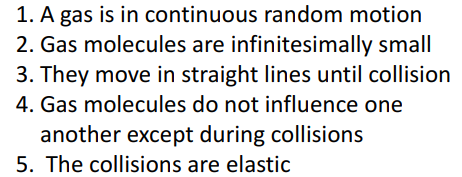
\includegraphics[width=0.8\textwidth]{KMT_slide.png}
		\caption*{\footnotesize{Prerequisites of KMT shown in slides\footnote{\tiny{Sun, Ting, \textit{CHEM2100J-FA21-Ch5-6}, pp. 35.}}}}
	\end{figure}
\end{frame}
\begin{frame}{Understanding from A New Point of View}
	Now we conclude
	\begin{itemize}
		\item \textcolor{gray}{A gas is in continuous random motion} and
			evenly distributed throughout the container. Irregular molecular 
			movement does not do work.
		\item Substances of the same chemical properties have the same particle size, 
			shape and functions.
		\item \textcolor{gray}{Gas molecules are infinitesimally small and they move in straight 
			lines until collision.}
		\item \textcolor{gray}{Gas molecules do not influence one another except 
			during collisions.}
		\item \textcolor{gray}{The collisions are elastic.}
	\end{itemize}
\end{frame}
\begin{frame}{Understanding from A New Point of View}
	\textbf{Example}
	\par For a model satisfying KMT, suppose there exists $N$ gas molecules in a cubic box with length $L$. Each molecule has the mass of $m$,
	 and the speed of $u$.	 
	\begin{figure}[!htbp]
		\centering
		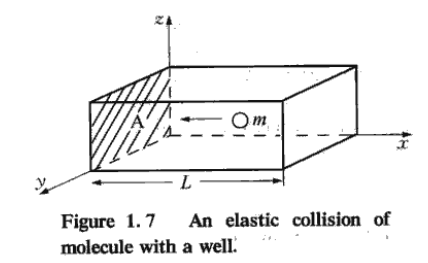
\includegraphics[width=0.5\textwidth]{KMT.png}
	\end{figure}
\end{frame}
\begin{frame}{Understanding from A New Point of View}
	(1) Calculate the average kinetic energy of each molecule $\bar{E_k}$.
	(2) If the relationship between average molecule and the temperature is
		\begin{equation*}
			\bar{E_k} = \frac{3}{2}kT
		\end{equation*}
		where $k$ denotes the Boltzmann constant and satisfies $k = \frac{R}{N_A}$.
\end{frame}
\begin{frame}{Understanding from A New Point of View}
	\textbf{Solution}
	\par We may assume there are $\frac{N}{3}$ molecules moving along the $x$-axis direction
	since there are $N$ molecules and only three directions in total. 
	\par Apparently, the momentum of these moleclues is $mu$. For a whole collision process 
	(we can also refer this process as $bouncing$), the distance the molecule travels is $2L$
	and the change of momentum is $2mu$.
\end{frame}
\begin{frame}{Understanding from A New Point of View}
	\textbf{(Continued)}
	\par Hence 
\end{frame}

\begin{frame}{Liquid}

\end{frame}

% -----------------------------------------------------------------------------

\section{Practical Functions}

\subsection{Blocks}
\begin{frame}{An example of blocks}
	\begin{block}{example}
		This is an example of block.
	\end{block}
	\begin{block}{}
		This is another block.
	\end{block}
\end{frame}

\subsection{Figures and Tables}
\begin{frame}{Examples of figures and tables}
	\begin{figure}
		\centering
		
\includegraphics[width=0.5\textwidth]{umji.png}
		\caption{An example of figure}
		\label{fig:demofig-1}
	\end{figure}
\end{frame}

\subsection{Graphs}
\begin{frame}{Examples of Graphs}
	\[ \xymatrix{
			A \ar[r] & B \ar@(ur,dr)
		} \]
	\[ \xymatrix{
			A \ar@<.5ex>[r]^{f} & \ar@<.5ex>[l]^{g} B
		} \]
	\[ \xymatrix@ru{
			A \ar[r] & B \ar[d] \\
			C \ar[u] & D \ar[l]
		} \]

\end{frame}

%------------------------------------------------------------------------------

\section{Conclusions}

\subsection{As for States of Matter}
\begin{frame}{Remarks}
	\begin{itemize}
		\item You can never be too careful about \textcolor{red}{UNITS}.
		\item Smoot's Legacy \url{http://alum.mit.edu/news/AlumniNews/Archive/smoots_legacy}.
		\item Smoot Salute! \url{http://web.mit.edu/spotlight/smoot-salute}.
	\end{itemize}
\end{frame}

% -----------------------------------------------------------------------------

\end{document}